\section{Theorie}
\label{sec:Theorie}

% In knapper Form sind die physikalischen Grundlagen des Versuches, des Messverfahrens, sowie sämtliche für die Auswertung erforderlichen Gleichungen darzustellen. (Keine Herleitung)

% (eventuell die Aufgaben)

% Der Versuchsaufbau: Beschreibung des Versuchs und der Funktionsweise (mit Skizze/Bild/Foto)

\begin{figure}
    \centering
    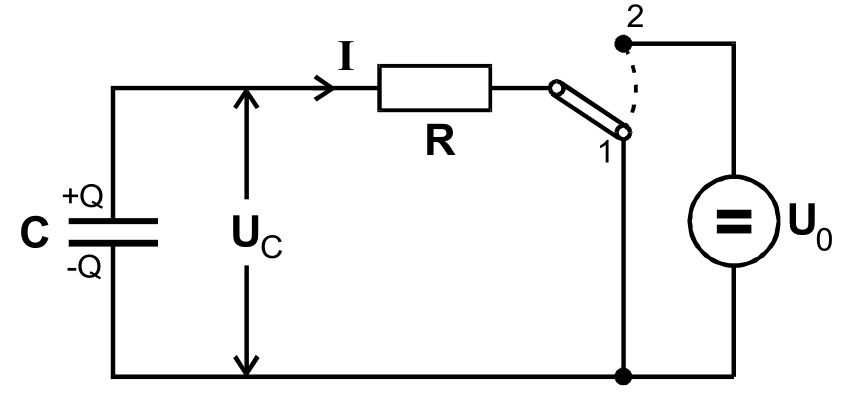
\includegraphics[width=\textwidth/2]{images/schaltung_1.png}
    \caption{Schaltbild eines RC-Kreises, der in Stellung 1 entladen und in Stellung 2 geladen wird. \cite{V353}}
    \label{fig:schaltung_1}
\end{figure}

Wenn ein System durch eine Änderung aus seinem Anfangszustand entfernt wird und daraufhin nicht-oszillatorisch in diesen zurückkehrt, kann man Relaxationseffekte beobachten. In \autoref{fig:schaltung_1} sind zwei dieser Relaxationsphänomene zu beobachten, das Auf- und Entladen eines Kondensators über einen Widerstand. 
Befindet sich der Schalter in \autoref{fig:schaltung_1} in Stellung eins, so entlädt sich der Kondensator mit der Kapazität $C$. Auf seinen beiden Platten liegt die Ladung Gesamtladung $Q$. Dadurch liegt zwischen den beiden Kondensatorplatten eine Spannung von 

\begin{equation}
    \label{eq:kondensatorspannung}
    U_C = \frac{Q}{C}.
\end{equation}

Durch das ohmsche Gesetz ist bekannt, dass durch diese Spannung $U_C$ und den Widerstand $R$ ein Strom 

\begin{equation}
    \label{eq:ohmschesgesetz}
    I = \frac{U_C}{R}
\end{equation}

erzeugt wird. 
Der zeitliche Verlauf der Ladung $Q$ auf dem Kondensator $C$ kann durch eine Exponentialfunktion beschrieben werden, dadurch ergibt sich

\begin{equation}
    \label{eq:entladungsladung}
    Q (t) = Q (0) \exp{\left(\frac{-t}{RC} \right)}.
\end{equation}

Wobei $RC$ eine Zeitkonstante ist, die im nächsten Abschnitt näher erklärt wird. \cite{V353}
Äquivalent dazu lässt sich der Aufladevorgang eines Kondensators $C$ durch die Spannung $U_0$ über den Widerstand $R$ beschreiben. Hierbei gelten folgende Randbedingungen für $Q$

\begin{align}
    \label{eq:ladung}
    Q (0) = 0 && Q (\infty) = C \cdot U_0.
\end{align}

Damit lässt sich der Aufladevorgang durch

\begin{equation}
    \label{eq:aufladungsladung}
    Q (t) = C \cdot U_0  (1- \exp{\left(\frac{-t}{RC} \right)} )
\end{equation}

beschreiben. \cite{V353} Dabei ist $RC$ wieder die Zeitkonstante aus \autoref{eq:entladungsladung}, mit dieser Konstante kann beschrieben werden, wie schnell sich ein System zu seinem Endzustand begibt. $RC$ ist festgeschrieben. Nachdem eine Zeit von 
\begin{equation}
    \Delta T = RC
\end{equation} verstrichen ist, ändert sich die Kondensatorladung $Q$ um den Faktor
\begin{equation}
    \label{eq:RC}
    \frac{Q (t = RC)}{Q (0)} = \frac{1}{e} \approx 0.386.
\end{equation}

Eine periodische Auslenkunge aus der Gleichgewichtslage erzeugt ebenfalls Relaxationsphänomene und kann ebenfalls mit einem RC-Kreis beschrieben werden. 

\begin{figure}
    \centering
    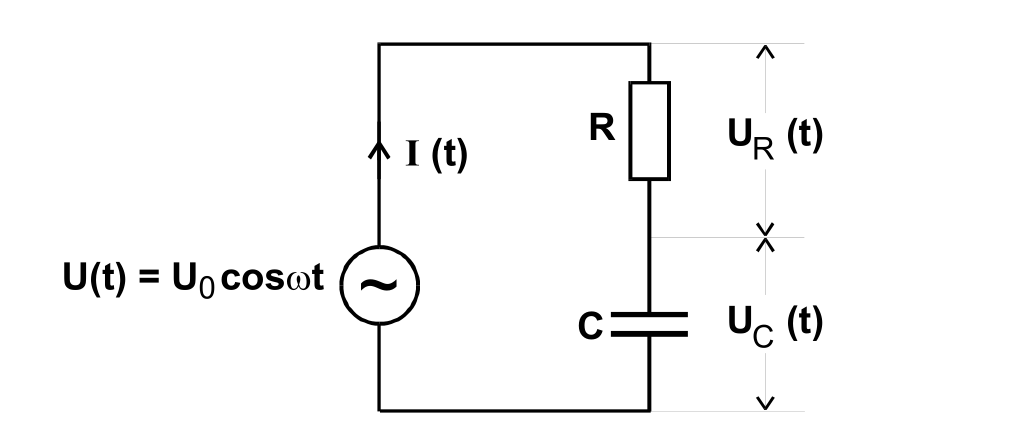
\includegraphics[width=\textwidth/2]{images/schaltung_2.png}
    \caption{Mögliches Schaltbild zur Entstehung eines Relaxationsphänomens durch periodische Anregung.  \cite{V353}}
    \label{fig:schaltung_2}
\end{figure}

Wird \autoref{fig:schaltung_2} durch die Wechselspannung $U (t)$ mit der Kreisfrequenz $\omega$ angetrieben, also 

\begin{equation}
    \label{eq:wechselspannung}
    U (t) = U_0 \cdot \cos \left(\omega t \right),
\end{equation}

ergeben sich für verschiedene $\omega$ andere Effekte. Für $\omega \ll \frac{1}{RC}$ werden die Kondensatorspannung $U_C$ und die Generatorspannung $U (t)$ \autoref{eq:wechselspannung} etwa gleich sein, da der Kondensator genug Zeit hat sich vollständig aufzuladen, bevor die Spannung wieder abfällt und ihr Vorzeichen ändert. Bei entsprechend höheren Frequenzen kann der Aufladevorgang nicht mehr vollständig stattfinden und die Amplitude $A$ der Kondensatorspannung wird kleiner werden. Sie ist gegeben durch

\begin{equation}
    \label{eq:amplitude}
    A (\omega) = \frac{U_0}{\sqrt{1 + \omega^2 R^2 C^2}}.
\end{equation}

Durch die verzögerte Aufladung entsteht eine Phasenverschiebung $\varphi$, die sich bei ansteigender Frequenz asymptotisch dem Wert $\varphi = \frac{\pi}{2}$ annähert. Wie an

\begin{equation}
    \label{eq:phasenverschiebung}
    \varphi (\omega) = \arctan \left(-\omega R C \right)
\end{equation}

auch zu erkennen ist. Aus allen bisher genannten Eigenschaften besitzt die Schaltung \autoref{fig:schaltung_2} die Eigenschaften eines Tiefpasses. \cite{V353}
Die RC-Kreis \autoref{fig:schaltung_2} besitzt noch eine weitere Eigenschaft, sie kann als ein sogenannter Integrator verwendet werden. Für $\omega \gg \frac{1}{RC}$ gilt folgende Beziehung

\begin{align}
    \label{eq:integrator}
    U (t) = RC \: \frac{\mathrm{d} U_C}{\mathrm{d}t}  && U_C (t) = \frac{1}{RC} \int _0^t U (t') \mathrm{d} t'
\end{align}

Dadurch wird zu der Generatorspannung $U (t)$ eine Stammfunktion $U_C (t)$ erzeugt, die sich nur durch einen Faktor unterscheidet. \cite{V353}

\subsection{Aufgaben}
\label{sec:aufgaben}



